
\documentclass[12pt]{article} %[epsf]
\usepackage{amsmath}
\usepackage[toc, page]{appendix}
\usepackage{graphicx}
\usepackage{caption}
\usepackage{subcaption}
\usepackage{hyperref}


\sloppy

\title{Realistic calorimeter hit digitisation in the {\tt ILDCaloDigi} processor}

\author{Daniel Jeans, The University of Tokyo,\\
Oskar Hartbrich, DESY.
}


\date{\today}

\begin{document}

\maketitle

\begin{abstract}

Description of quasi-realistic calorimeter hit digitisation in ILD, as implemented in
the {\tt ILDCaloDigi} processor in the {\tt MarlinReco} package.

\end{abstract}


\section{Introduction}

Possibilities for more realistic treatment of calorimeter hits from silicon-- and scintillator--based calorimeters have been 
implemented in the {\tt ILDCaloDigi} processor within {\tt MarlinReco}. The aim of these is to allow the study of the effects 
of various detector ``defects'' such as mis-calibrations, limited dynamic ranges, and signal fluctuations, 
and also to allow more robust comparisons between technologies under more realistic conditions.
This notes discusses the implementation as defined by rev. 4777 of the {\tt MarlinReco} package, available at
{\tt https://svnsrv.desy.de/viewvc/marlinreco/MarlinReco/}.

The energy of {\tt SimCalorimeterHits} produced by the {\tt Mokka} simulation is the energy deposited in the detection
element (silicon or scintillator) as calculated by {\tt GEANT4}. They therefore take account of Landau fluctuations
in the energy deposits.
The role of the digitisation is to simulate the behaviour of the process which converts this energy deposit into the 
reconstructed energy of hits used in detector reconstruction: this includes effects due to the detection medium
(e.g. creation of electron-hole pairs in silicon), 
the readout system (e.g. pixelated photo-detectors (PPD - SiPM/MPPC)) used to readout scintillation light,
and the electronics which treat these signals (e.g. limited dynamic range).

This note describes a parameterised model which to model such effects. The parameters to be used should be decided by
the detector groups, by comparing to data collected during test beam campaigns.

{\tt ILDCaloDigi} also applies a threshold on the energy of hits, as well as possibilities for requirements on the timing
of energy deposits. This pre-existing functionality was extended from the original {\tt ILDCaloDigi} on some points.

\section{General}

The various effects implemented for realistic digitisation are controlled by parameters of the {\tt ILDCaloDigi}
processor which can be set at run time via the {\tt Marlin} steering file (i.e. without recompiling).
Most parameters are duplicated, with one set for the ECAL, and the other for the HCAL, allowing different
parameters to be used for the each of the systems. In this note, we denote there duplicated parameters as ``*\S CAL*'':
``\S'' should be replace by ``E'' for the ECAL, and ``H'' for the HCAL.

Which type of digitisation to apply to ECAL hits is controlled by the {\tt ECAL\_apply\_realistic\_digi} parameter: a value of
0 (the default) turns off the realistic effects described in this note, and a value of 1 (2) applies the silicon--
(scintillator--) specific effects. 
In the case of the scintillator HCAL, the parameter {\tt HCAL\_apply\_realistic\_digi}
plays a similar role, with a value of 0 (1) turning off (on) the simulation of realistic digitisation effects.

Several digitisation parameters are specified in terms of MIP units, so the {\tt ILDCaloDigi} processor requires 
factors with which to convert the deposited energy (in GeV) to MIP units: these are passed by the {\tt Calib\S CALMIP} parameters.

Various detector parameters are taken from the {\tt gear} file, in particular the layer layout and number of virtual 
cells per scintillator strip in the case of a scintillator strip-based ECAL. 
If these are not available in the {\tt gear} file, they can be specified via the
parameters {\tt ECAL\_default\_layerConfig} and {\tt StripEcal\_default\_nVirtualCells} (if values {\em are} found in the 
{\tt gear} file, they take precedence over the value of these parameters).

\section{Timing and energy thresholds}
Mokka provides a list of single energy deposition contributions from Geant4, including deposited energy in GeV and time stamp in ns for each active detector volume (cell or strip). To increase realism of the simulation, cuts on energy and timing of these hits can be applied.

\subsection{Energy threshold}
Hits in once detector cell are only kept after the digitisation stage if the hit amplitude is above a threshold. This threshold can be configured by the {\tt \S calThreshold} steering parameters. 
The unit used for interpreting the given threshold is chosen by setting {\tt \S CALThresholdUnit} to either 
{\tt GeV} for deposited energy in GeV (default), 
{\tt MIP} for deposited energy in MIP equivalents, or 
{\tt px} for deposited energy in SiPM pixels. 
{\tt MIP} and {\tt px} require appropriate settings of the digitisation parameters explained in \autoref{sec:scintdigi}.

\subsection{Hit timing}
\textbf{It is imperative to run the preceding Mokka simulation with {\tt /Mokka/init/lcioDetailedShowerMode true}.}
Otherwise, detailed subhit information will not be stored to the output file, which is necessary for hit timing 
selections to work properly (see also \cite{SG_HcalOpt}).

Two different algorithms for hit timing selection can be chosen via {\tt \S CALSimpleTimingCut}.

If {\tt \S CALSimpleTimingCut} is {\tt true}, all hit contributions with hit time between 
{\tt \S CALTimeWindowMin} and {\tt \S CALBarrelTimeWindowMax}/{\tt \S CALEndcapTimeWindowMax} 
are summed into the digitised hit. The hit time of the output is set to the earliest subhit 
within that time window. This timing mode resembles test beam measurements with the CALICE 
physics prototypes using external trigger and a fixed acquisition time window.

If {\tt \S CALSimpleTimingCut} is {\tt false}, a more complex algorithm is applied. 
It aims to cluster hits in time into windows of {\tt \S CALDeltaTimeHitResolution} 
and generates individual output hits for each of these time clusters. This may be useful 
to simulate more complex aqcuisition electronics, but needs very careful setup of parameters. 
Especially the SPIROC chip currently used in the CALICE AHCAL and ScECAL prototypes cannot be well 
modeled by this. Also with the current implementation, it is possible to lose contributions 
within the general time window defined by {\tt \S CALTimeWindowMin} and {\tt \S CALTimeWindowMax}. 
It is thus advised to use {\tt \S CALSimpleTimingCut true} at the moment.


\section{Technology-blind effects}
\label{sec:common}

\subsection{Mis-calibrations}
The effect of imperfect energy calibrations can be simulated by the use of the parameters
{\tt \S CAL\_miscalibration\_uncorrel} and {\tt \S CAL\_miscalibration\_correl}, which causes hit energies to
be smeared as 
\begin{equation*}
\begin{split}
E' = & E \times \\
& \text{\tt RandGauss} ( 1, \text{\tt \S CAL\_miscalibration\_uncorrel}) \times \\
& \text{\tt RandGauss} ( 1, \text{\tt \S CAL\_miscalibration\_correl}) ,
\end{split}
\end{equation*}
where $\text{\tt RandGauss} (\mu, \sigma)$ represents a random number taken from a Gaussian distribution of mean $\mu$ and 
standard deviation $\sigma$. In the case of {\tt \S CAL\_miscalibration\_uncorrel}, a new random number is taken for each 
calorimeter hit (simulating completely uncorrelated mis-calibrations), 
while in the case of {\tt \S CAL\_miscalibration\_correl}, a single random number is used for all \S CAL 
hits in a given event (simulating completely correlated mis-calibrations).

The uncorrelated miscalibrations induced by {\tt \S CAL\_miscalibration\_uncorrel} of each detector cell can be chosen to be either 
the same from event to event, or newly chosen for each event. 
This is controlled by setting the parameter {\tt \S CAL\_miscalibration\_uncorrel\_memorise = true} or {\tt false} respectively.
The first approach is closer to reality, however in the case of a calorimeter with many cells, can lead to large memory consumption;
in the case of typical physics events randomly spread across the whole ILD detector, the second, more memory-efficient, 
approach is almost certainly sufficient. The first approach is probably only necessary in the case of repeated injection into the same detector
region, as occurs, for example, in test beams.

\subsection{Dead detector cells}
The effect of dead detector cells can be simulated by use of the parameter {\tt \S CAL\_deadCellRate}, which causes the energy
of hits to be set to zero if a random number taken from a uniform distribution in the range [0, 1] is smaller than the 
value of the {\tt \S CAL\_deadCellRate} parameter.
Similar to the miscalibration effects, the parameter {\tt \S CAL\_deadCell\_memorise} selects whether dead cells are randomised for each event or constant for the whole run.

\subsection{Dynamic range of readout electronics}
The saturation of the readout electronics can be simulated by setting the parameter {\tt \S CAL\_maxDynamicRange\_MIP},
in which case the energy of the hit is limited to this value of this parameter (specified in MIP units):
\begin{equation*}
E'_{MIP} = min ( \text{\tt \S CAL\_maxDynamicRange\_MIP}, E_{MIP} ).
\end{equation*}

\subsection{Noise}
Uncorrelated, random noise can be simulated by the parameter {\tt \S CAL\_elec\_noise\_mips}, which
alters the hit energy by
\begin{equation*}
E'_{MIP} = E_{MIP} + \text{\tt RandGaus} ( 0, {\tt \S CAL\_elec\_noise\_mips} ).
\end{equation*}

\section{Silicon ECAL hits}

A rather simple approach is followed in the case of silicon readout: 
the energy deposit in the silicon is converted into a number of electron-hole (e-h) pairs,
using the parameter {\tt energyPerEHpair} which gives the energy required to create an e-h pair (in eV).
This number of e-h pairs is then used to define the mean of a Poisson distribution, from which a random number is taken 
to get a statistically smeared number of e-h pairs. 
This approach is an over-simplification: it ignores, for example, the Fano
effect which reduces the fluctuation of e-h pairs with respect to this simple Poisson approximation.
Since these fluctuations are anyway much smaller than the Landau fluctuations in energy deposit, 
they have an almost negligible effect.

\section{Scintillator hits}
\label{sec:scintdigi}


In the case of the scintillator \S CAL, several effects are included: non-uniformity of response along the strip length,
and the finite number of photo-electrons and PPD pixels. 
These processes typically have much larger effects than in the case of silicon-based readout.
For the scintillator-based HCAL, the same effects, except the strip non-uniformity, are included. 
The names of the relevant parameters for the HCAL have ``{\tt ECAL\_}'' replaced by ``{\tt HCAL\_}''.

\subsection*{Non-uniformity along strip length}
In Mokka simulation, ECAL scintillator strips can be split along their length into virtual cells, 
in each of which a {\tt SimCalorimeterHit} can be produced. 
ILDCaloDigi identifies all virtual-cell hits coming from the same strip, and combines them into a single {\tt CalorimeterHit}.
Different weights can be given to the energies of different virtual cells within a strip, to simulate non-uniformity
along the strip length. A simple exponential dependence has been implemented, controlled by the parameter
{\tt ECAL\_strip\_absorbtionLength}. The energy of the final {\tt CalorimeterHit} is then given by
\begin{equation*}
E'_{MIP} = \sum_{i} E_{i} \times exp( \delta x_i / \text{\tt ECAL\_strip\_absorbtionLength} )
\end{equation*}
where the index $i$ runs over the virtual cells of a strip, and $\delta x_i$ is the distance between the 
centres of the virtual cell and the strip. This energy is then treated in the following steps:

\subsection*{Conversion of energy to MIP equivalents}
The deposited energy in the scintillator is converted to MIP units using the parameter {\tt Calib\S CALMIP}
\begin{equation*}
E_{MIP} = \text{\tt Calib\S CALMIP} \times E_{GeV} .
\end{equation*}

\subsection*{Finite number of photo-electrons and PPD pixels}
A finite number of photo-electrons (p.e.) are produced in the PPD by energy deposited in the scintillator.
The energy deposited in the scintillator is converted to an average number of photo-electrons in the PPD:
\begin{equation*}
n_{pe}^{ave} = E_{MIP} \times \text{\tt \S CAL\_PPD\_PE\_per\_MIP},
\end{equation*}.

The finite number of PPD pixels introduces both a saturation effect on the average response and additional signal fluctuations relevant mostly at high signal levels. 
To include these statistical effects in photon generation and PPD response two separate models have been proposed, called here the \emph{Stoykov Model} and the \emph{Binomial Model}. Both proposed models of PPD response ignore cross-talk between pixels, after pulses, and similar effects.

\subsubsection*{Stoykov Model}
The \emph{Stoykov Model} follows the calculation steps in \cite{PPD}, by first quantising the number of photons hitting the PPD by taking the actual number of p.e. $n_{pe}$ randomly from a Poisson distribution with mean $n_{pe}^{ave}$. Using a Poisson distribution is justified, as from the around 4500 photons generated per incident MIP \cite{JGU_LA} only around 15 (depending on the chosen {\tt \S CAL\_PPD\_PE\_per\_MIP}) actually fire pixels in the PPD.

The average number of fired PPD pixels ${n}_{pix}^{ave}$ for a given number of input p.e. $n_{pe}$ is modeled as
\begin{equation*}
{n}_{pix}^{ave} = \text{\tt \S CAL\_PPD\_N\_Pixels} \times ( 1 - exp ( -n_{pe} / \text{\tt \S CAL\_PPD\_N\_Pixels}  ) ), 
\end{equation*}
and fluctuations in the number of fired PPD pixels due to the limited number of pixels are modeled as \cite{PPD}:
\begin{equation*}
\begin{split}
n_{pix} = & {n}_{pix}^{ave} + \delta n, \text{ where} \\
\delta n = & \text{\tt RandGauss}( 0, w ) \\
       w = & \sqrt{\text{\tt \S CAL\_PPD\_N\_Pixels} \times exp(-\alpha) \times ( 1 - (1+\alpha) \times \exp ( - \alpha ) ) } \\
       \alpha = & n_{pix}^{ave} / \text{\tt \S CAL\_PPD\_N\_Pixels}
\end{split}
\end{equation*}

The terms given above are derived using an approximation of longer terms. The validity of this approximation is shown in \ref{sec:variance_para}.
Modelling this fluctuation with a Gaussian shape is somewhat problematic, as it should not be possible to fire more PPD pixels than the number of incident photons.

\subsubsection*{Binomial Model}
In the \emph{Binomial Model}, first the average number of fired PPD pixels is calculated as 
\begin{equation*}
{n}_{pix}^{ave} = \text{\tt \S CAL\_PPD\_N\_Pixels} \times ( 1 - exp ( -n_{pe}^{ave} / \text{\tt \S CAL\_PPD\_N\_Pixels}  ) ), 
\end{equation*}.

This mean amplitude is then quantised by randomising it from a binomial distribution with $n=\text{\tt \S CAL\_PPD\_N\_Pixels}$ and $p=\frac{{n}_{pix}^{ave}}{\text{\tt \S CAL\_PPD\_N\_Pixels}}$

While the \emph{Stoykov Model} is intuitive in its succession of steps, it suffers from the unknown shape of the fluctuation from finite PPD pixels. The \emph{Binomial Model} is less intuitive in its approach, but has been successfully used in the digitisation of AHCAL physics prototype simulations.

In appendix \autoref{sec:paracomp} it is shown that the expected resolutions arising from these digitisations are exactly identical for both models. As the \emph{Binomial Model} does not suffer the shape problems of the \emph{Stoykov Model}, the \emph{Binoial Model} is used in this processor.

\subsection*{Variations in pixel response}
Variations in individual pixel signals (due to e.g. variations in capacitance) can be simulated by using the parameter
\text{\tt \S CAL\_pixel\_spread}, which introduces extra variations in the PPD signal $n_{pe}^{sig}$
\begin{equation*}
n_{pix}^{sig} = n_{pix} \times \text{\tt RandGauss} ( 1, \text{\tt \S CAL\_pixel\_spread} / \sqrt( n_{pix} ) ).
\end{equation*}

\subsection*{Electronics noise}
Electronics noise is then added to $n_{pix}^{sig}$, as described in section \ref{sec:common}.

\subsection*{Mis-calibration of total pixel number, unfolding of average PPD response}
A mis-calibration in this number of 
total PPD pixels can be introduced by the parameter {\tt \S CAL\_PPD\_N\_Pixels\_uncertainty}, in which
case the assumed number of PPD pixels is defined to be:
\begin{equation*}
N_{pix} = \text{\tt \S CAL\_PPD\_N\_Pixels} \times 
\text{\tt RandGauss}(1, \text{\tt \S CAL\_PPD\_N\_Pixels\_uncertainty}).
\end{equation*}

This mis-calibrated number of total pixels is then used to 
unfold the PPD response by using the inverse of the saturation curve.
If the fraction of fired pixels $r$ is less than 95\%, the unfolding is done as
\begin{equation*}
n_{pe}^\text{unfold} = - N_{pix} \times log ( 1 - n_{pix}^{sig} / N_{pix} ) ),
\end{equation*}
while if $r > 0.95$,  a linearised approximation is used:
%      npe = 1/(1-r)*(npe-r*smearedNpix)-smearedNpix*std::log(1-r);
\begin{equation*}
n_{pe}^\text{unfold} =  
(n_{pix}^{sig} - r \times N_{pix})/(1-r) - n_{pix}^{sig} \times log ( 1 - r ).
\end{equation*}

%where $\epsilon = 1$ is a small number which ensures that the logarithm is well behaved.



\subsection*{Conversion back to energy}
The unfolded number of p.e. is then converted back into a scintillator energy deposit using the parameters
{\tt \S CAL\_PPD\_PE\_per\_MIP}
and 
{\tt Calib\S CALMIP}.

\section{Conclusion}
Possibilities for realistic modeling of silicon-- and scintillator--based calorimeter  energy readout have been
implemented in {\tt ILDCaloDigi}. The modeling is rather simple, but should be adequate to allow 
a comparably realistic simulation of the different technologies. 
Tuning of the processor parameters
should be performed by comparisons with data collected by detector prototypes in test beams.

\begin{appendices}

\section{Comparison of parametrisation models}
\label{sec:paracomp}
We define $a$ as the number of photons hitting the SiPM, $n$ as the number of different SiPM pixels hit from these $a$ photons and the number of total SiPM pixels $m$. Furthermore $p={}^n/_{m}$ denotes the fraction of fired SiPM pixels.
The relation between incoming photons (unsatured signal) and fired pixels (saturated response) is given by
\begin{align}
	n = f_{sat}(a) &= me^{-\frac{a}{m}} \\
	a = f_{sat}^{-1}(n) &= -m \log\left(1-\frac{n}{m}\right) \\
	\frac{\mathrm{d}{f_{sat}^{-1}(n)}}{\mathrm{d}n} &= m\frac{1}{m-n} = e^\frac{a}{m}.
\end{align}


Beginning with the variance of the binomial distribution:
\begin{align}
	\mathrm{Var}^{bino}_{sat} &= mp(1-p) \\
	&= m \left( \frac{n}{m} \right) \left(1-\frac{n}{m}\right) \nonumber \\
	&= m \left(e^{-\frac{a}{m}}\right)\left(1-e^{-\frac{a}{m}}\right)
\end{align}

Converting to the unsaturated variance, following \cite{PPD}:
\begin{align}
	\mathrm{Var}^{bino}_{unsat} &= \mathrm{Var}^{bino}_{sat}\left(\frac{\mathrm{d}{f_{sat}^{-1}(n)}}{\mathrm{d}n}\right)^2 \\
	&= m \left(e^{-\frac{a}{m}}\right)\left(1-e^{-\frac{a}{m}}\right)\left(e^{\frac{2a}{m}}\right) \nonumber \\
	&= m\left(e^{\frac{a}{m}}-1\right)
\end{align}

This yields the resolution of the binomial SiPM model:
\begin{equation}
	\mathrm{Res}^{bino} = \frac{\sqrt{\mathrm{Var}^{bino}_{unsat}}}{a} = \frac{\sqrt{m\left(e^{\frac{a}{m}}-1\right)}}{a}
\end{equation}

It is easily seen, that this is equivalent to the parametrised resolution $\mathrm{Reso}^{Stoykov}$ given in \cite{PPD}:
\begin{align}
	\mathrm{Res}^{Stoykov} &= \frac{1}{\sqrt{m}}\sqrt{\frac{1}{\alpha}+\left(\frac{1}{\alpha}\sqrt{e^\alpha-1-\alpha}\right)^2},\quad \alpha = \frac{a}{m} \\
	&= \frac{1}{\sqrt{m}}\sqrt{\frac{m}{a}\left(1+\left(\frac{m}{a}\left(e^\frac{a}{m}-1-\frac{a}{m}\right)\right)\right)} \nonumber \\
	&= \frac{\sqrt{m\left(e^\frac{a}{m}-1\right)}}{a} = \mathrm{Res}^{bino}
\end{align}


\section{Full vs. approximate Variance \cite{PPD}}
\label{sec:variance_para}
In \cite{PPD} the variance of the number N of urns containing one or more balls after randomly distributing $a$ (photons) balls into $m$ urns (pixels) is given as
\begin{equation}
	\mathrm{Var}^{Stoykov} = m(m-1)(1-2m^{-1})^a+m(1-m^{-1})^a-m^2(1-m^{-1})^{2a}.
\end{equation}
This is claimed to be approximated by the shorter form
\begin{equation}
	\mathrm{Var}^{Stoykov}_{approx} = m(1-e^{\frac{a}{m}})
\end{equation}
for $m, n \rightarrow \infty$ and the ratio ${}^a/_m$ bounded. 

To check the validity of these assumptions, a simple comparison was performed for a sensor with $m=2000$ pixels. As shown in \autoref{fig:variance}, the difference between the full and approximate variance terms are very small for amplitudes \textgreater 10 pixels. Even for amplitudes \text1ess 0px the observed mismatch is far from relevant, as for the full resolution Poissonian uncertainty is added in quadrature, which is orders of magnitude larger for such amplitudes. Additionally, a threshold of $0.5$\,MIP (corresponding to about $7.5$\,pixels fired) is expected for ILD operation. Thus low amplitude hits are not taken into account at all.

From this we conclude, that the approximate variance form is suitable for use in digitisation.
\begin{figure}
        \centering
        \begin{subfigure}[b]{0.5\textwidth}
                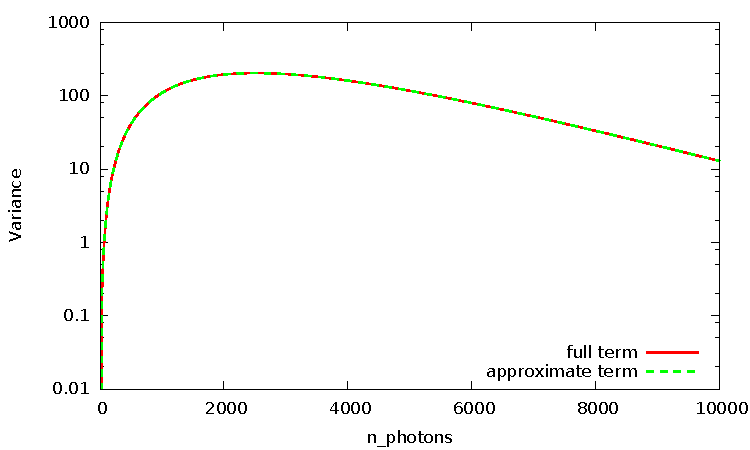
\includegraphics[width=\textwidth]{fig/comp_variance/variance}
                \caption{Variance, full amplitude range}
                \label{fig:var_full}
        \end{subfigure}%
        ~ %add desired spacing between images, e. g. ~, \quad, \qquad, \hfill etc.
          %(or a blank line to force the subfigure onto a new line)
        \begin{subfigure}[b]{0.5\textwidth}
                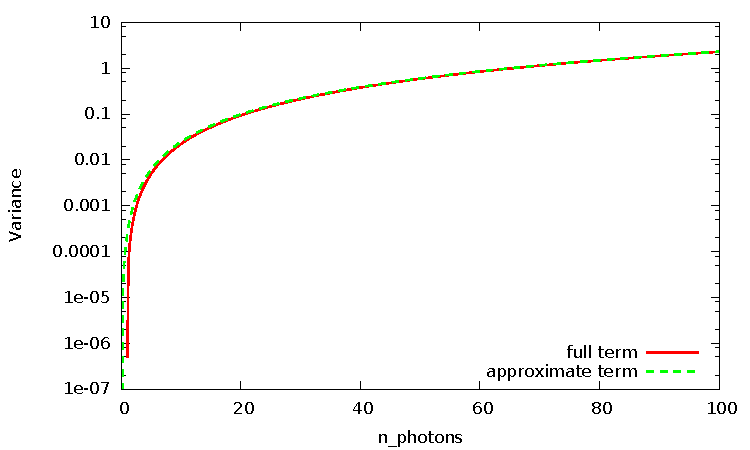
\includegraphics[width=\textwidth]{fig/comp_variance/variance_zoom}
                \caption{Variance, zoomed}
                \label{fig:var_zoom}
        \end{subfigure}
        \\
        \begin{subfigure}[b]{0.5\textwidth}
                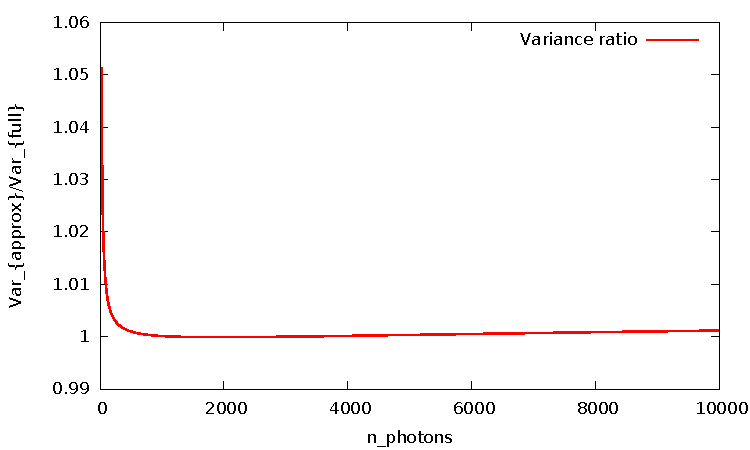
\includegraphics[width=\textwidth]{fig/comp_variance/ratio}
                \caption{Variance ratio, full amplitude range}
                \label{fig:ratio_full}
        \end{subfigure}%
        ~ %add desired spacing between images, e. g. ~, \quad, \qquad, \hfill etc.
          %(or a blank line to force the subfigure onto a new line)
        \begin{subfigure}[b]{0.5\textwidth}
                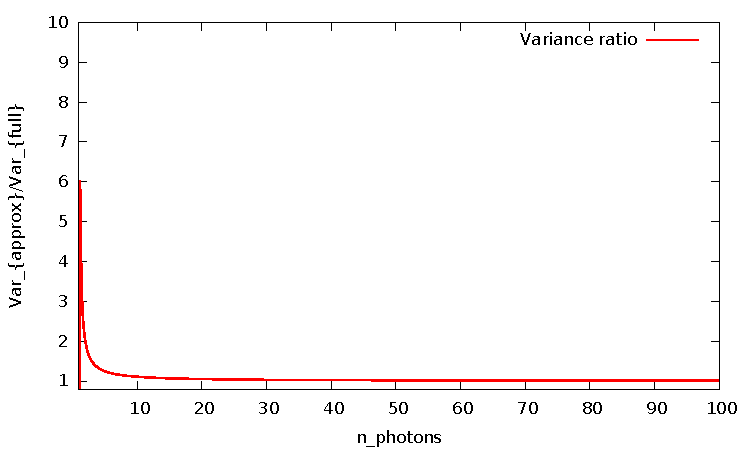
\includegraphics[width=\textwidth]{fig/comp_variance/ratio_zoom}
                \caption{Variance ratio, zoomed}
                \label{fig:ratio_zoom}
        \end{subfigure}
        \caption{Comparison of full and approximate variance terms as given in \cite{PPD}. Only for very small amplitudes  \textless 10\,pixels relevant deviations are visible.} \label{fig:variance}
\end{figure}
\end{appendices}

% \newpage

\begin{thebibliography}{99}
\bibitem{PPD}
A.Stoykov et al., ``On the limited amplitude resolution of multipixel Geiger-mode APDs", arXiv:0706.0746.
\bibitem{JGU_LA}
Lennart Adam, Uni Mainz, private communication with OH, 27.01.2015
\bibitem{SG_HcalOpt}
Steven Green, Cambridge, presentation for ILD optimisation meeting: https://indico.cern.ch/event/369380/contribution/3/material/slides/0.pdf

\end{thebibliography}

\end{document}

